\section{Design Motivation}
\textit{Crossfire} has three main design goals: multiprocess support, remote and
mobile debug, and cross-browser debugging. These closely related goals arose out
of an interplay between user benefit and development costs. As an open source
project we must work with development resources motivated by goals: no matter
how much value Firebug users may receive from a goal, the selection must be
limited by the motivation of open source contributors.

Necessity motivated the first \textit{Crossfire} design goal, multiprocess
support. Soon after the Google Chrome browser was released, the Firefox team at
Mozilla began plans to convert Firefox to a multi-process design.  The Google
browser uses one controlling process for the application and one process for
each Web page.  This allows the browser to use the operating system isolation to
prevent problems on one page from bringing down the entire application and it
allows each page to use a different physical processor on modern multi-core
computers \cite{GoogleChrome}.  Depending upon the Firefox browser platform
changes, a shift to multiprocess could render Firebug unusable.

 As a practical
matter we could not wait for the new platform to become available: with only
two full-time developers plus a number of dedicated but part-time contributors,
and a commitment to continuous compatibility with Firefox we had to begin work
immediately to ensure that our small resource could complete the transition in
time to remain a viable project.

Therefore we assumed that Firefox would eventually adopt
an architecture similar to Google Chrome: a client/server split debugger with a
back-end in one process and a front-end in another process.  We believe
that this assumption is planning for the worst case: converting Firebug to
client/server is a multi-person-year effort but likely to work with what
ever the Firefox team decides to do.

While necessity forced our action, opportunity followed. The client/server
choice, if successful, adds two new dimensions to Firebug for users: remote
debug and mobile device debug. We expect the value of these dimensions to grow
as more developers work in distributed teams and as mobile plays an increasingly
important role in Web application development.  In fact this value was
recognized by the DragonFly Web debugger for Opera well before even the Google
Chrome browser. The additional cost of designing for remote and mobile debug
on top of a client/server design -- primarily mechanisms for specifying the
connection addresses -- comes with potentially high benefits.  Moreover, the
benefits align with directions important to the project's primary open source
contributors (one full time person from IBM and Mozilla).

The final goal of cross-browser debugging offers even more benefits to
Firebug users.  Web application developers by definition target all Web users,
but not all Web users are running identical Web platforms. Almost all
potential users of a Web site will be running one of few similar but slightly
different browsers. The commonality allows Web developers to do most of their
work on one browser, then test for differences on other browsers. Of course in
the latter case they need to debug the problem on a browser with unfamiliar debugging
tools. A common debugging tool across the major browsers would help with this
common and significant problem.

The benefit of cross-browser debugging comes at a high cost for the project.
Instead of one server and one client, we face at minimum one server for every
browser. And for each server we have to deal with both the slight differences in
browser implementation of standard Web APIs and potential large differences in
how debuggers can connect to the browser.


Unlike commercial or pure research projects, a community-driven open source
project like Firebug might balance the cost of implementing cross-browser debugging support by
attracting more contributors interested in this particular goal. That is, by
adding this costly goal we can attract new contributors, allowing us to create
more total value. In particular new contributors from the Orion
project\cite{orion}, joined to create a \textit{Crossfire} server for Microsoft
Internet Explorer and from the Eclipse project\cite{EclipseJSDT} to create a new
\textit{Crossfire} client in Java for connecting to Eclipse. Moreover, a
cross-browser client for Web debugging can be largely implemented with Firebug
Lite code, allowing our project to consolidate developer resources around fewer
lines of code to maintain.


Our three design goals created constraints for the \textit{Crossfire}
implementation. Above we outlined how the multiprocess support lead to a
client-server design choice. Support for remote and mobile debug forces
isolation of user interface to the client (excepting some small interface for
connection specification). The cross-browser goal creates constraints
indirectly: to minimize the extra cost of supporting multiple servers we chose
to adopt the Google Chrome communications channel (sockets) and wire protocol
format (JSON). Neither Firefox nor Internet Explorer had existing servers, so
they did not alter our choices. Opera had a server but no one on our open source
team planned to work with Opera and the server itself was not open source making
implementation more difficult.  Since Firebug is already written in JavaScript,
JSON format is especially easy to work with and has good performance\cite{json}.
 For the communications protocol, HTTP would be a better choice for the project:
the JavaScript support for HTTP is much better than sockets and HTTP works
better in practical remote scenarios through firewalls.  However we made the
judgment that better socket support was coming in future\cite{websocketapi},
support was adequate now, and lowering cost on a Google Chrome back-end was
important.  In addition our goals imply that the client and the communication
protocol should be built from open Web standards to maximize the reuse across
servers.

\section{Evolution not Revolution}
In addition to motivating developers to contribute to \textit{Crossfire}, we
also need to motivate users to help us test and refine the system. As a
practical project supporting 3 million users, Firebug provides a large base of
experienced Web developers working with a broad spectrum of Web technologies. An
open source, working, state-of-the-art debugger motivates users to explain
problems, create test cases, provide documentation and to help other users with
problems that come up. To harness this
 unusual resource  for \textit{Crossfire} we need a plan for incremental
 refactoring of Firebug to be compatible
with \textit{Crossfire}.  The refactoring plan needs to provide waypoints for
the development and it needs to provide intermediate value to users and/or
contributors.


\subsection{Inter-application JavaScript Debugging}
The first intermediate state for \textit{Crossfire} is shown in Fig.\ref{fig:fireclipse}.
\begin{figure}[htp]
  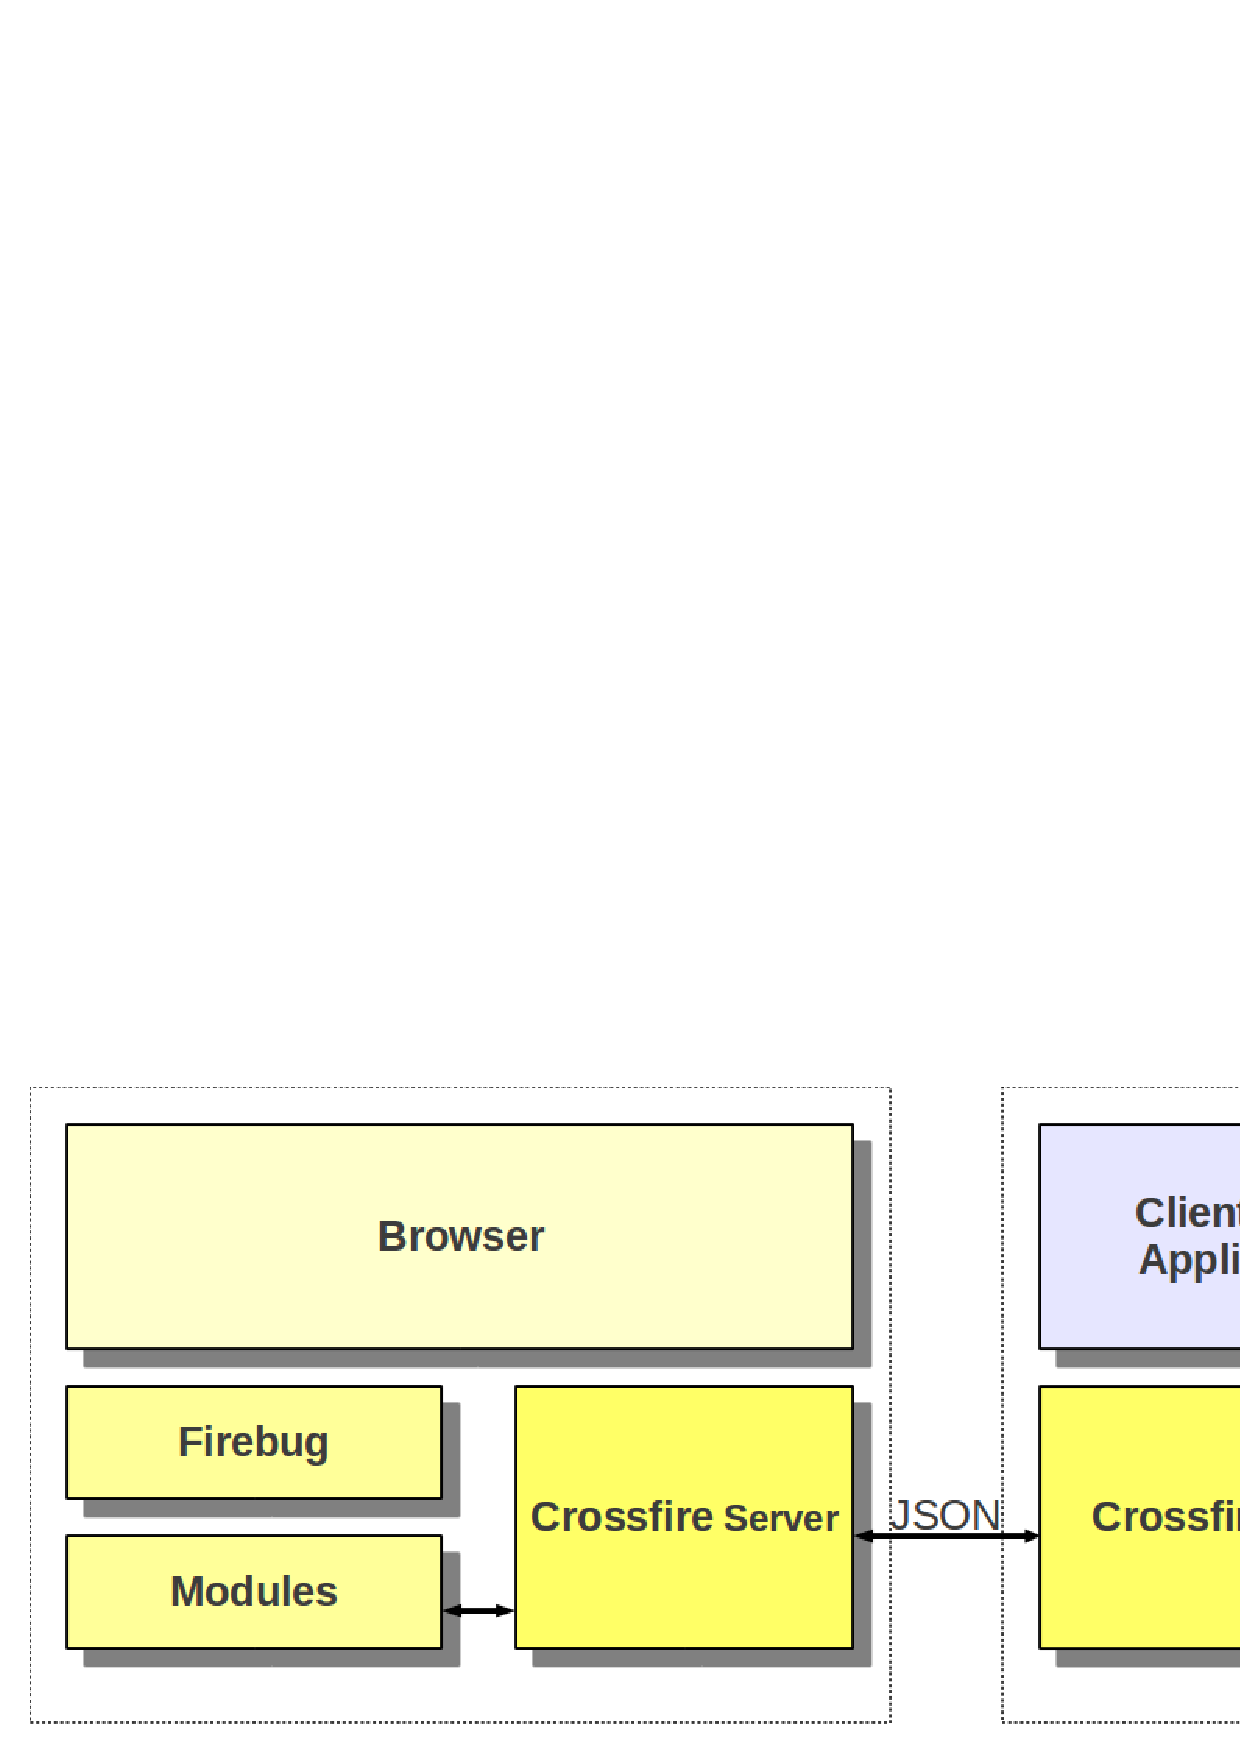
\includegraphics  [width = 86 mm] {figures/fireclipse.png}
  \caption{Inter-application JavaScript Debugging \textit{Crossfire} architecture.
\textit{Crossfire} versions 0.1 to 0.3 connected to an Eclipse plugin, supporting simple JavaScript debugging}
 \label{fig:fireclipse}
\end{figure}
In Firefox we implemented a \textit{Crossfire} server limited to support for JavaScript debugging.
In Eclipse we implemented a \textit{Crossfire} client. This allows the user interface in Eclipse to control
 and examine the JavaScript program running
in Firefox.  A proprietary version of the client shipped in IBM's Rational
Application Developer product for two years, then the open source Eclipse team created a new implementation as part of it's JavaScript Developer
Tools (JSDT) project\cite{EclipseJSDT}.  By working towards the Eclipse team's
goals of remote JavaScript debugging, this stage of the work provided valuable implementation
experience and engagement with the Eclipse team.
This work is largely complete.

\subsection{Intra-browser JavaScript Debugging}
The second intermediate state implements the client side of the JavaScript part
of \textit{Crossfire} in a Web browser as sketched in Fig.~\ref{fig:fbugChrome}.
\begin{figure}[htp]
  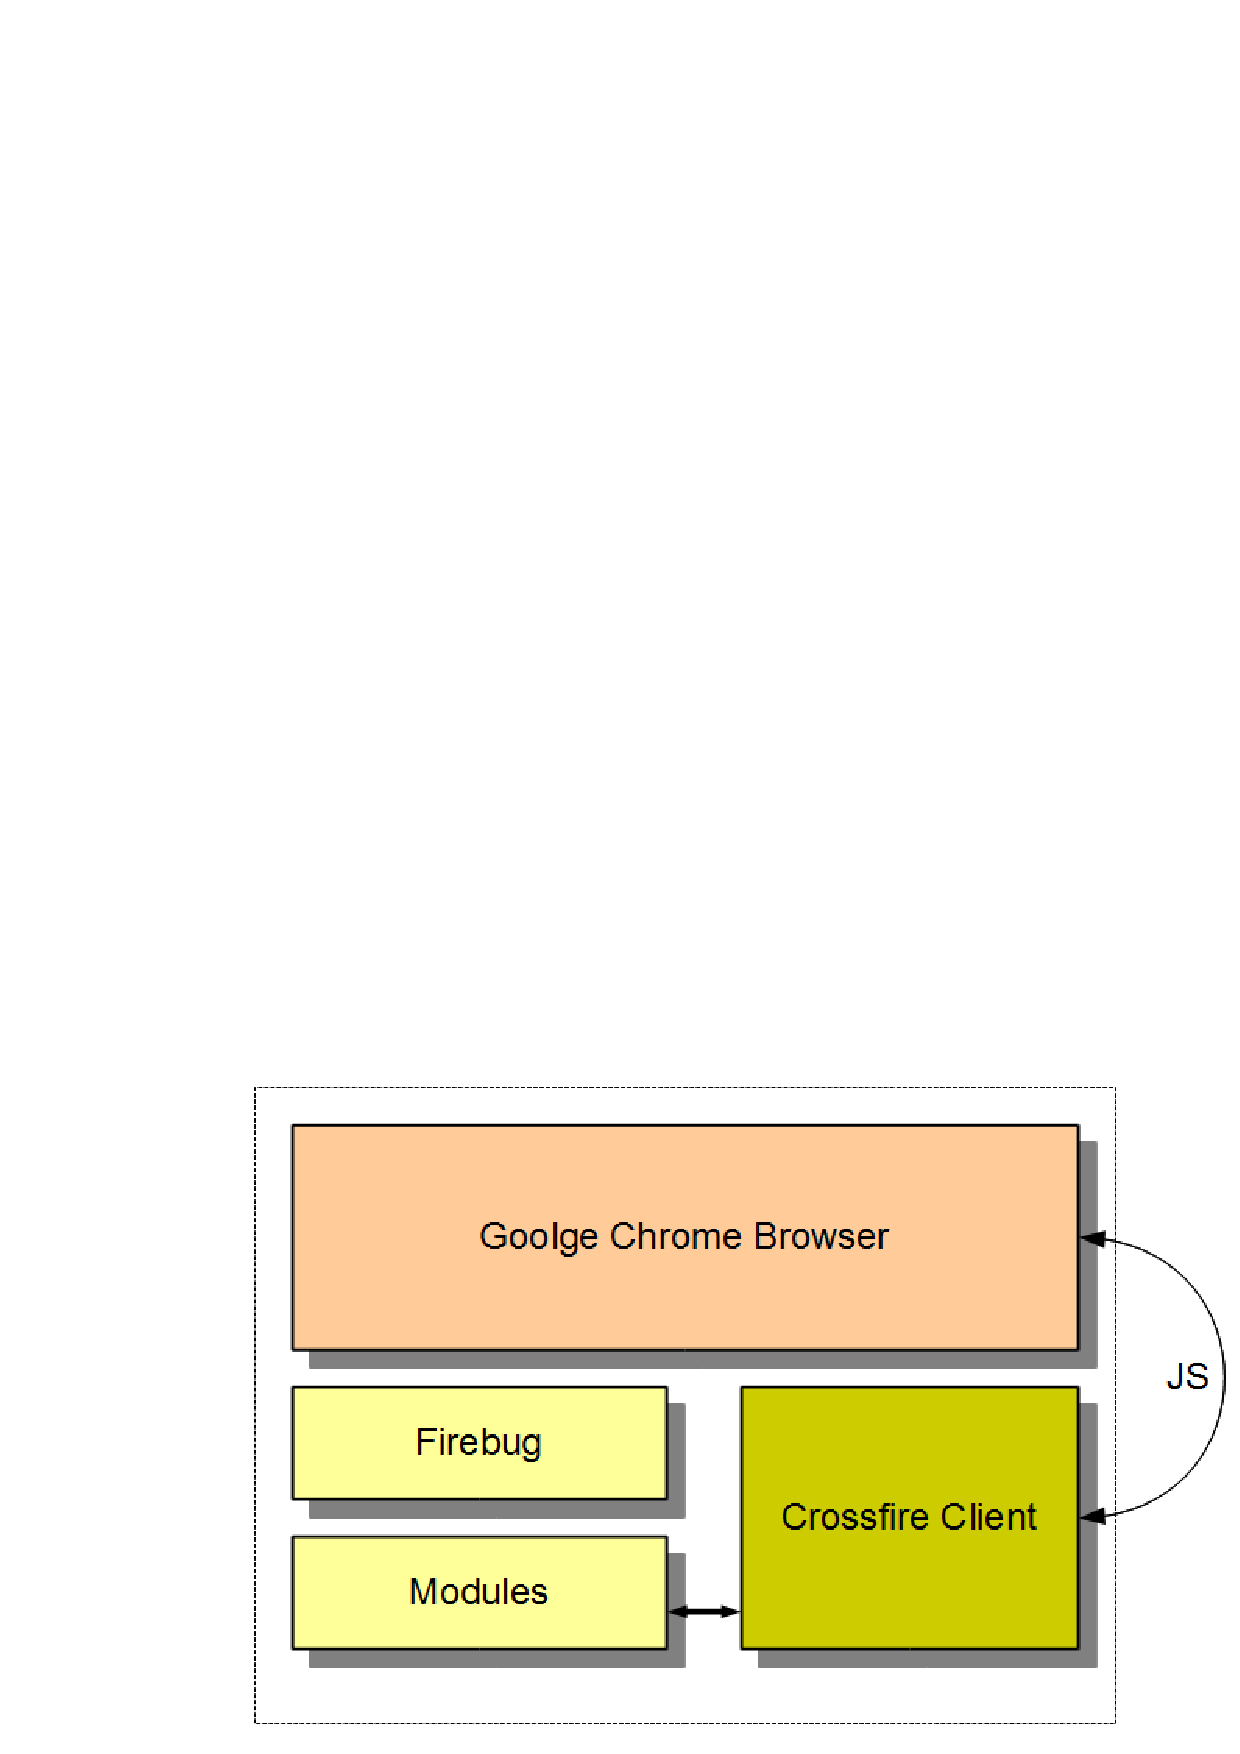
\includegraphics  [width = 86 mm] {figures/fbugChrome.png}
  \caption{Intra-browser JavaScript Debugging \textit{Crossfire} architecture.
\textit{Crossfire} versions 0.4 targets supporting simple JavaScript debugging with the client and server in the same application.}
 \label{fig:fbugChrome}
\end{figure}
While this diagram seems a bit bizarre, with the debugger running in and
connecting back into the the same browser, this step allows us to add JavaScript
debug support to the Firebug Lite implementation in the Google Chrome browser
while we simultaneously refactor the Firefox  \textit{Crossfire} server to
resemble the Google Chrome back end.


The key reason this architecture makes sense is that a large part of the
non-JavaScript parts of a Web page debugger uses standard Web APIs. That  means
that three different applications, Firebug Lite running as co-resident with a
Web page, Firebug Lite running as a Google Chrome extension,  and the
HTML/CSS/Console debug support code in Firebug for Firefox can use identical
code in different wrappers. By re-engineering our current somewhat divergent
code to group the identical parts we reduce maintainence. By adding for
JavaScript debugging using the newly platform-independent Firefox code to the
Firebug for Google Chrome code we add user value: the beginnings of cross
browser development. Both efforts contribute to our final goals.


Furthermore, the two JavaScript-only \textit{Crossfire} servers, one for Firefox
and one for Google Chrome, will be able to support alternative clients. In
particular, the Orion project, a Web based Web-development system, plans to
support JavaScript debugging over \textit{Crossfire} on their editor user
interface. In return that project is implementing a \textit{Crossfire} server
for Internet Explorer, allowing us to cover more than 75\% of the browser market
with \textit{Crossfire} supported tools. This work is scheduled to complete in
June, 2011.


\subsection{Cross-browser Debugging}
The final stage completes the transformation of an in-process single browser Web
page debugger to a client-server cross-browser tool as shown in
Fig.~\ref{fig:crossbrowser}. \begin{figure}[htp]
  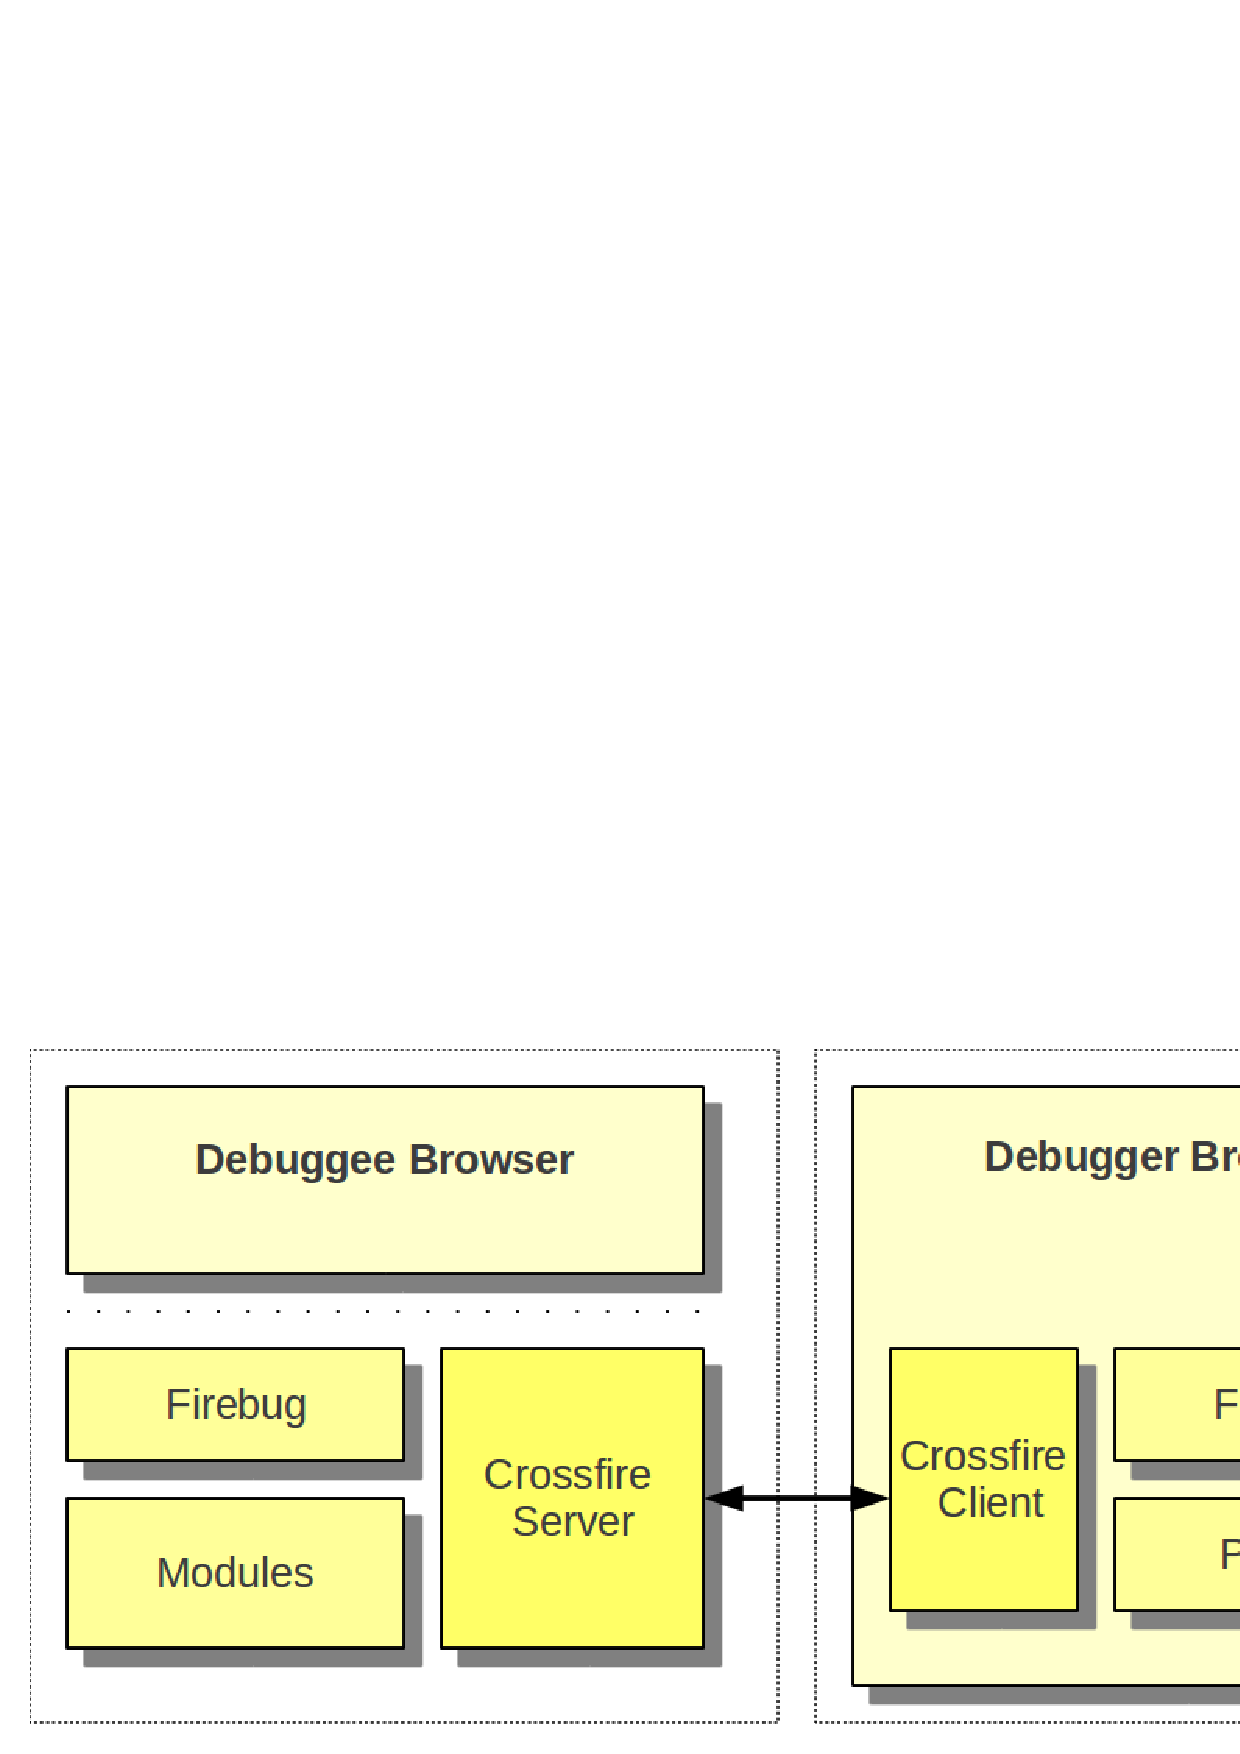
\includegraphics  [width = 86 mm] {figures/crossbrowser.png}
  \caption{Cross-browser Debugging architecture, proposed.}
 \label{fig:crossbrowser}
\end{figure}
Conceptually we simply re-apply the approach ironed out in the previous step to
the rest of the program and arrive at the complete value proposed at the outset.
In practice, the concept hides a lot of work. Lots of lines of code must be
carefully divide into two piles and the whole must get working again. This work
is scheduled to complete in Dec. 2011.

\subsection{Modules and Tools Interface}
In parallel with the architectural changes outlined above, we also need to make
important infrastructure improvements. Two such improvements are of particular
interest: conversion of the source code to 'modules' and introduction of a
cross-browser JavaScript tools application programming interface.


\paragraph{Modules} The original Firebug for Firefox and Firebug Lite code used
HTML \texttt{<script>} tags to load and compile the source. This approach has
two major drawbacks: 1) all of the top-level symbols in each file mix with the
top-level symbols of any other files loaded in the same scope and 2) the
load/compile steps are serialized. The first drawback never affected Firebug
code because all of the files encapsulated their symbols in function scope. But
the second one means that loading code always causes an upfront overhead to
starting the application.


A replacement for  \texttt{<script>} tag loading will need to support both
client and server sides of a refactored Firebug and it must allow us to debug
our own code.  As in other cases, we also want a solution that avoids additional
work by the development team. The solution we adopted was
\textit{RequireJS}\cite{requirejs}, a form of a module loader inspired by the
CommonJS\cite{commonjs} open standards effort.  For the client side or Firebug
Lite we can use this loader directly once we change our source to its format.
For the server side we needed to implement code to read within the Firefox
platform and support debugging.


\paragraph{Tools Interface}
During the transformation from monolithic to client-server application, Firebug
needs to operate in both modes. The obvious way to deal with this is to
introduce a programming interface between the front and back ends. In Firebug
for Firefox, the interface functions call the back end directly; in the
intermediate and initial releases of the cross-browser version these functions
call the \textit{Crossfire} client API.  Similarly in the back end, the
multiprocess versions of the interface call the \textit{Crossfire} server.
Notice that this interface becomes a natural programming layer for interaction
between parts of the debugger. Since \textit{Crossfire} is designed to be
cross-browser, with some care in the design, the programming interface we create
becomes a general purpose Tools Interface for open Web development.


The module and Tools Interface infrastructures complement one another. Each
logical chunk of the Tools Interface corresponds to the exported symbols from
one of the modules and the conditional assembly of the application from modules,
to become either in-process or client-server, works by using the module loader
to select the appropriate implementations of the interface.

